\section{Vetores no Espaço}
\begin{frame}[label=vetores]{O conjunto  $\R^3$}
Denotamos por   $\R^3$ o conjunto formado pelas {\color{blue}triplas ordenadas} $(x,y,z)$ tais $x$, $y$ e $z$ são números reais.
\medskip

Podemos representar geometricamente os elementos de $\R^3$ usando um {\color{blue}sistema de coordenadas cartesianas}, que consiste na escolha de três  eixos com a mesma origem, $OX$, $OY$ e $OZ$, mutuamente perpendiculares e que a orientação positiva é escolhida de acordo com a {\color{blue} regra da mão direita}.

\begin{center}
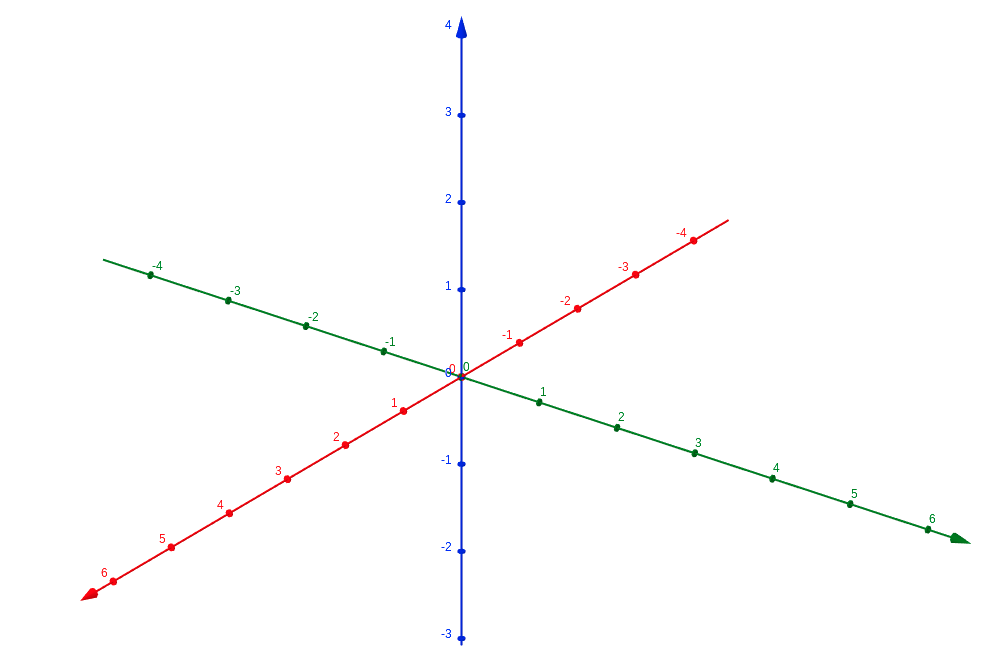
\includegraphics[scale=0.2]{figuras/eixos3d2.png}
\end{center}
\end{frame}


\begin{frame}[label=vetores]

\begin{exe}
\begin{enumerate}
\item Determine os pontos $(1,3,1)$ e $(3,-2,2)$ no sistema cartesiano.
\item Esboce o conjunto dos pontos que satisfazem a equação $z=3$.
\end{enumerate}
\end{exe}


\end{frame}


\begin{frame}[label=vetores]{Vetores no $\R^3$}
O conjunto $\R^3$ torna-se um espaço vetorial quando o munimos com as seguintes  operações: Se $\vec{u}=(u_1,u_2,u_3)$,  $\vec{v}=(v_1,v_2,v_2)$ e $\alpha\in \R$ então
\[\vec{u}+\vec{v}=(u_1+v_1,u_2+v_2,u_3+v_3),\]
\[\alpha \vec{v}=(\alpha v_1,\alpha v_2,\alpha v_3).\]
Neste caso, o {\color{blue}vetor nulo} é $\vec{0}=(0,0,0)$ e o {\color{blue}simétrico} de $\vec{v}$ é  $-\vec{v}=(-v_1,-v_2,-v_3)$.

\begin{center}
\begin{minipage}{0.7\textwidth}
\begin{block}{}
Se {\color{red}$A=(a_1,a_2,a_3)$} e {\color{red}$B=(b_1,b_2,b_3)$} então
\[{\color{red}\overrightarrow{AB}}={\color{blue}\vec{u}=(b_1-a_1,b_2-a_2,b_3-a_3)}.\]
\end{block}
\end{minipage}
\end{center}
\end{frame}


\begin{frame}[label=vetores]
Do mesmo modo,
\begin{center}
\begin{minipage}{0.7\textwidth}
\begin{block}{}
\[\|{\color{red}\overrightarrow{AB}}\|=\sqrt{{\color{blue}(b_1-a_1)^2+(b_2-a_2)^2 +(b_3-a_3)^2}}.\]
\end{block}
\end{minipage}
\end{center}


\begin{exe}
Dados $A=(0,3,1)$, $B=(2,3-1)$ e $C=(0,1,0)$ determine $2\vt{AB}+\vt{AC}$.
\end{exe}


\end{frame}

\subsection*{Vetores no $\R^n$}
\begin{frame}[label=vetores]{Vetores no $\R^n$}

De modo geral, denotamos por   $\R^n$ o conjunto formado pelas {\color{blue} $n$-uplas ordenadas} $(x_1,x_2,\ldots,x_n)$ tais $x_i\in \R$ para todo $i=1,2,\ldots,n$.
\medskip

O conjunto $\R^n$ torna-se um espaço vetorial quando o munimos com as seguintes  operações: Se $\vec{u}=(u_1,u_2,\ldots,u_n)$,  $\vec{v}=(v_1,v_2,\ldots,v_n)$ e $\alpha\in \R$ então
\[\vec{u}+\vec{v}=(u_1+v_1,u_2+v_2,\ldots,u_n+v_n),\]
\[\alpha \vec{v}=(\alpha v_1,\alpha v_2,\ldots,\alpha v_n).\]
Neste caso, o {\color{blue}vetor nulo} é $\vec{0}=(0,0,\ldots,0)$ e o {\color{blue}simétrico} de $\vec{v}$ é  $-\vec{v}=(-v_1,-v_2,\ldots,-v_n)$.

\begin{center}
\begin{minipage}{0.7\textwidth}
\begin{block}{}
Se {\color{red}$A=(a_1,a_2,\ldots,a_n)$} e {\color{red}$B=(b_1,b_2,\ldots,b_n)$} então
\[{\color{red}\overrightarrow{AB}}={\color{blue}\vec{u}=(b_1-a_1,b_2-a_2,\ldots,b_n-a_n)}.\]
\end{block}
\end{minipage}
\end{center}

\end{frame}

\begin{frame}[label=vetores]
De forma análoga, também definimos a {\color{blue} norma (ou comprimento)} de um vetor do $\R^n$ por
\begin{center}
\begin{minipage}{0.7\textwidth}
\begin{block}{}
Se {\color{blue}$\vec{u}=(u_1,u_2,\ldots,u_n)$} então
\[{\color{blue}\vec{u}=\sqrt{u_1^2+u_2^2+\ldots+u_n^2}}.\]
\end{block}
\end{minipage}
\end{center}

Um {\color{blue} vetor unitário} é um vetor que tem norma 1. Dado qualquer vetor não nulo $\vec{v}$, sempre podemos obter um {\color{blue}vetor unitário} $\vec{u}$ com mesmo sentido de $\vec{v}$, basta fazer
\[\vec{u}=\frac{1}{\|\vec{v}\|}\vec{v}.\]
Esse processo é chamada de {\color{blue} normalização} de $\vec{v}$. Alguns textos usam a notação $\hat{v}$ e o chamam de {\color{blue}versor}.


\end{frame}

\begin{frame}[label=vetores]


\begin{exe}
Normalize o vetor $\vec{v}=(2,-1,3)$.
\end{exe}


\begin{casa}
Normalize os vetores $\vec{u}=(1,\sqrt{2},\sqrt{3},0)$ e $\vec{v}=(4,-\sqrt{2},0,-5)$.
\end{casa}
\end{frame}




\begin{frame}[label=vetores,fragile=singleslide]{Combinação Linear}

\begin{defin}
Um vetor $\vec{v}\in \R^n$ é uma {\color{blue} combinação linear} de vetores $\vec{v}_1, \vec{v}_2, \ldots, \vec{v}_k$ se existem escalares $\alpha_1,\alpha_2,\ldots, \alpha_k$ tais que
\[\vec{v}=\alpha_1\vec{v}_1+\alpha_2\vec{v}_2+\cdots +\alpha_k\vec{v}_k.\]
\end{defin}

\begin{pycode} 
import sympy as sp

x1,x2,x3,x4=sp.symbols('x_1 x_2 x_3 x_4',real=True)
X=sp.Matrix([x1,x2,x3,x4])
def pt(Y):
 return((Y[0],Y[1],Y[2],Y[3]))

v1=sp.Matrix([0.14,0.08,0,1.6])
v2=sp.Matrix([0.58,0,0,0])
v3=sp.Matrix([0.15,1.3,26,6.9])
v4=sp.Matrix([0,0.08,38,0.2])
B=sp.Matrix([3,1.1,60,11])
\end{pycode} 

No exemplo anterior, escrevemos  o vetor $\vec{v}=\pyl{B}$ como combinação linear dos vetores
\[\vec{v}_1=\pyl{v1},\ \vec{v}_2=\pyl{v2},\ \vec{v}_3=\pyl{v3},\ \text{ e } \vec{v}_4=\pyl{v4}. \]

\end{frame}
